\chapter{Theoretical Foundation}
\label{chap:02_foundation}


This chapter provides the theoretical foundation to understand concepts that will be used in this thesis. First, the concept of Scalability is described. Second, the theory behind a deployment pipeline is explained. Third, the concept of autonomic computing is  introduced. Fourth, the theory of measuring system performance is explained. Lastly, the concept of monitoring is being described.


\section{Scalability}
\label{sec:02_foundations_scalability}
% What is scalability
Scalability defines the ability of a computing system to handle an increasing amount of load \cite{Farcic2017Toolkit21}. 
% Limit of scalability
The limit of scalability is reached when a computing system cannot serve the requests of its concurrent users \cite{Wilder2012CloudPatterns}.
% Vertical and horizontal
Different approaches exist to increase the scalability of a system. The two main approaches are vertical scaling and horizontal scaling.


\subsection{Horizontal Scaling}
\label{subsec:02_foundations_scalability_horizontal-scaling}
% What is horizontal scaling
Horizontal scaling is accomplished by adding nodes to the computing environment to increase the overall capacity.
Each node typically adds an equal amount of computing capacity (e.g., amount of memory) \cite{Wilder2012CloudPatterns}.
% DIstribution
By increasing the number of nodes in a computing environment, the workload can be distributed more efficiently across all nodes to handle and balance an increasing workload \cite{Wilder2012CloudPatterns, Abbott2015ScalabilityArt}.


% Limit of hor scaling
Scaling a computing environment horizontally is limited by the efficiency of each added node.
% The simplicity of homo nodes
The horizontal scaling approach is more efficient with the simplicity of homogeneous nodes.
% Homogeneous nodes
Homogeneous nodes add the same amount of computing power to the system and can perform the same work and response as other nodes.
% Examples
With homogeneous nodes, creating strategies for capacity planning, load balancing, and auto-scaling is more efficient.
% Different nodes
In an environment with different types of nodes, creating these strategies is more complex due to the need for context \cite{Wilder2012CloudPatterns}.


\subsection{Vertical Scaling}
\label{subsec:02_foundations_scalability_vertical-scaling}
% Concept
Vertical scaling refers to increasing the overall capacity by improving the computing power with additional hardware of individual nodes (e.g., adding memory, increasing number of CPU cores) \cite{Wilder2012CloudPatterns}.


% hardware capacity
If additional hardware has to be added to a system, it is not guaranteed that more powerful hardware is available or affordable.
% The limit of vertical scalability
Therefore, vertical scaling is limited by available hardware.
% Downtime
Additionally, changing the physical hardware of a running system can require a downtime. For most systems, a downtime should be avoided because it will interrupt important services running on the system \cite{Wilder2012CloudPatterns}.


% ===========================================
% ===========================================
\section{Deployment Pipeline}
\label{sec:02_depl-pipeline}
% Short Abstract
A deployment pipeline is an implementation of the process of getting software from source code to production.
% Based on CI
It is based on the concept of Continuous Integration (CI).
% Involves what
The process involves building, testing, and deploying software through automated scripts \cite{Farley2010CI}.


\subsection{Continuous Integration}
% Abtract def
Continuous Integration is a development practice where automated scripts validate each change on a primary codebase. This ensures that errors are detected and fixed in an early development stage \cite{Duvall2007CI}.
% What its about
The CI process is responsible for building and testing the software to guarantee that it is in a releasable state at all times \cite{Rossel2017CICD}.
% Advantages
CI contributes with the following advantages to the development life cycle of an application:
\begin{itemize}
\item Reduce risks:
The CI process runs tests and validates the software on each change. Errors are detected in an early stage and can be fixed immediately \cite{Duvall2007CI}.

\item Reduce manual processes:
% Same time
The CI process will perform every time a commit has been made to the code base.
% Same process
Each run is processed the same way every time.
% No human
Therefore, no human intervention is needed to start the process, which saves time and cost \cite{Duvall2007CI}.

\item Generate deployable software:
If an error occurs during a CI run, developers will be informed, and fixes can be applied immediately.
This ensures that the software is in a deployable state at all times \cite{Duvall2007CI}.
\end{itemize}


\subsection{Requirements of a Continuous Integration Process}
\label{sec:02_depl-pipeline_requirements}
% Requirements
The implementation of a CI process is based on several requirements:
% The list
\begin{enumerate}
\item Version control repository:
To manage changes to the code base, the source code and all other assets like the build script should be hosted on a single version control repository.
% Changes
Each change on the code base triggers the CI process on the build server to run against the latest version available \cite{Duvall2007CI}.

\item Build server:
The build server is responsible for monitoring the code base for changes.
% Execute
If a change is committed, the build server automatically executes the CI scripts in order \cite{Rossel2017CICD, Duvall2007CI}.

\item Build scripts:
This includes all automation scripts to validate the source code \cite{Duvall2007CI}. Typical examples are:
\begin{itemize}
\item Building the software binaries (e.g., \texttt{.jar} binaries for Java source code).
\item Running unit and integration tests.
\item Deploying the binaries to a test or production environment.
\end{itemize}
\end{enumerate}


\subsection{Continuous Integration Process Implementation Example}
% Explain workflow
\paragraph{}\Fig{fig:02_foundation_deployment_ci_scenario} demonstrates the CI scenario.
% Commit changes
First, a developer commits changes to the version control repository.
% CI
The CI server monitors the repository for changes. After the change has been committed, the CI server pulls the latest version of the source code and executes all build scripts in sequence to integrate the software.
% Feedback
Finally, the CI server sends feedback to inform the developer about the build script status  \cite{Duvall2007CI}.


% The scenario figure
\begin{figure}[h]
\centering
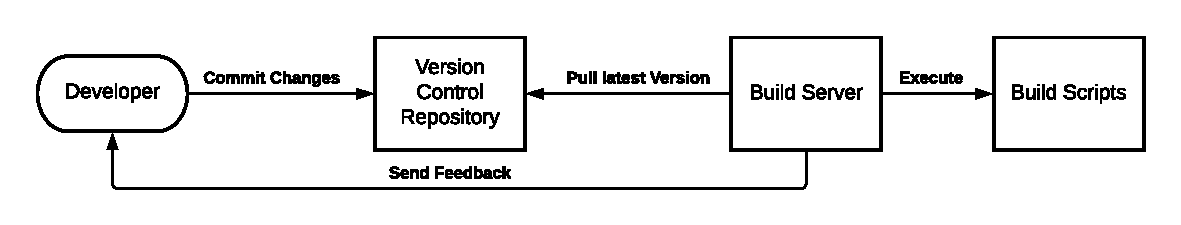
\includegraphics[scale=0.7]{images/02_theoretical_foundation/deployment_pipeline/ci_scenario}
\caption{Continuous Integration Scenario - Source: Authors own model, based on \cite{Duvall2007CI}.}
\label{fig:02_foundation_deployment_ci_scenario}
\end{figure}


% Explain build script order
\paragraph{}A CI run should be executed in a headless automated process. It is not feasible to rely on a manual process.
% Automated scripts
All assets to perform the CI run should be accessed from the repository. Therefore a machine can start the build script process by executing a command script in an automated fashion \cite{Duvall2007CI}.
% The example
An example of a logical build script order is illustrated in \Fig{fig:02_foundation_deployment_ci_script-order}.


% The build script order figure
\begin{figure}[h]
\centering
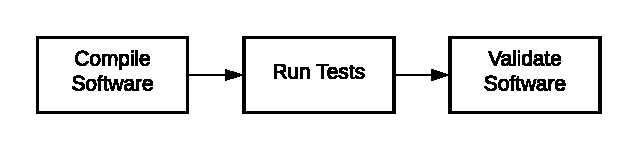
\includegraphics[scale=1]{images/02_theoretical_foundation/deployment_pipeline/ci_build_script_order}
\caption{An example of a logical build script order for a CI process- Source: Authors own model, based on \cite{Duvall2007CI}.}
\label{fig:02_foundation_deployment_ci_script-order}
\end{figure}


% ===========================================
% ===========================================
\section{Autonomic Computing}
\label{sec:02_ac}
% What is autonomic computing
Autonomic computing is the ability of an IT infrastructure to automatically manage itself according to high-level objectives defined by administrators \cite{Kephart2003VisionComputing}.
% Why
Autonomic computing gives an IT infrastructure the flexibility to adapt dynamic requirements quickly and effectively to meet the challenges of modern business needs \cite{Murch2004Autonomic}. Therefore, autonomic computing environments can reduce operating costs, lower failure rates, make systems more secure, and quickly respond to business needs \cite{Jacob2004AutonomicSolution}.


% What does it need
Computing systems need to obtain a detailed knowledge of its environment and how to extend its resources to be truly autonomous \cite{Murch2004Autonomic}.
% The 4 basic elements
An autonomic computing system is defined by four elements:
\begin{itemize}
\item Self-configuring:
Self-configuring refers to the ability of an IT environment to adapt dynamically to system changes and to be able to deploy new components automatically. Therefore, the system needs to understand and control the characteristics of a configurable item \cite{Murch2004Autonomic, Sinreich2006AnAB}.

\item Self-optimizing:
To ensure given goals and objectives, a self-optimizing environment can efficiently maximize resource allocation and utilization \cite{Jacob2004AutonomicSolution}. To accomplish this requirement, the environment must monitor all resources to determine if an action is needed \cite{Murch2004Autonomic}.

\item Self-healing:
Self-healing environments can detect problematic operations and then perform policy-based actions to ensure that the system's health is stable \cite{Sinreich2006AnAB, Jacob2004AutonomicSolution}. The actions' policies have to be defined and should be executed without disrupting the system \cite{Sinreich2006AnAB, Jacob2004AutonomicSolution}.

\item Self-protecting:
The environment must identify unauthorized access and threats to the system and automatically protect itself by taking appropriate actions during its runtime \cite{Sinreich2006AnAB, Jacob2004AutonomicSolution}.
\end{itemize}


\subsection{Autonomic Computing Concept}

% Concept figure
\begin{figure}[h]
\centering
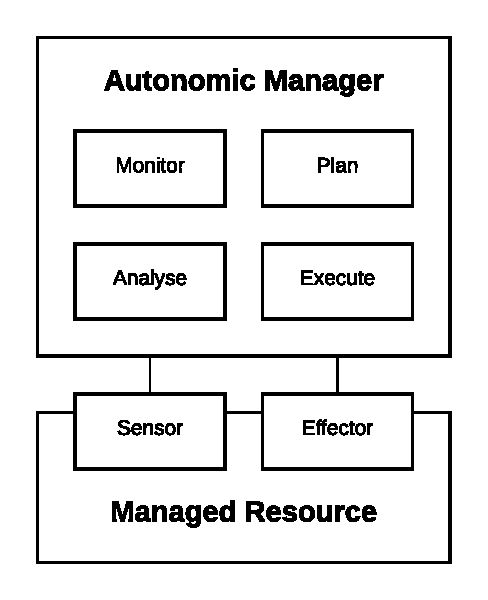
\includegraphics[scale=1]{images/02_theoretical_foundation/autonomic_computing/autonomic_computing_concept}
\caption{Autonomic computing concept - Source: Authors own model, based on \cite{Jacob2004AutonomicSolution}.}
\label{fig:ac_concept}
\end{figure}

% Figure + short description
\Fig{fig:ac_concept} demonstrates the main concept of an autonomic computing environment. The autonomic computing architecture relies on monitoring sensors and an adoption engine (autonomic manager) to manage resources in the environment \cite{Goscinski2011CloudComputing}.
% About the environment
In an autonomic computing environment, all components have to communicate with each other and can manage themselves. Appropriate decisions will be made by an autonomic manager that knows the given policies \cite{Jacob2004AutonomicSolution}.

% Control loop figure
\begin{figure}[h]
\centering
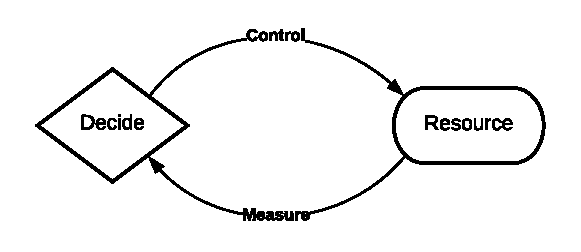
\includegraphics[scale=1]{images/02_theoretical_foundation/autonomic_computing/control_loop}
\caption{The control-loop concept - Source: Authors own model, based on \cite{Murch2004Autonomic}.}
\label{fig:ac_control_loop}
\end{figure}

% Explain control loop
The core element of the autonomic architecture is the control-loop. \Fig{fig:ac_control_loop} illustrates the concept of a control-loop. The control-loop collects details about resources through monitoring and makes decisions based on analysis of the collected details to adjust the system if needed \cite{Murch2004Autonomic}.


\subsection{Managed Resources}
\label{subsec:02_ac_resources}
% Figure
\begin{figure}[h]
\centering
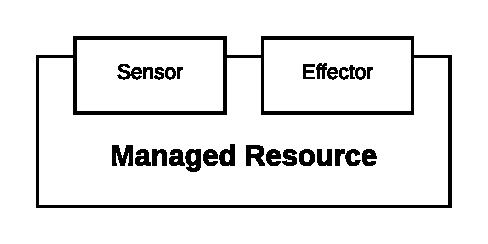
\includegraphics[scale=1]{images/02_theoretical_foundation/autonomic_computing/managed_resource}
\caption{Managed resource - Source: Authors own model, based on \cite{Jacob2004AutonomicSolution}.}
\label{fig:ac_managed_resource}
\end{figure}

% Explanation
A managed resource is a single component or a combination of components in the autonomic computing environment \cite{Murch2004Autonomic, Jacob2004AutonomicSolution}. A component can be a hardware or software component, e.g., a database, a server, an application, or a different entity \cite{Sinreich2006AnAB}.
% Sensors and Effectors
They are controlled by their sensors and effectors, as illustrated in \Fig{fig:ac_managed_resource}. Sensors are used to collect information about the state of the resource, and effectors can be used to change the state of the resource \cite{Jacob2004AutonomicSolution}. The combination of sensors and effectors is called a touchpoint, which provides an interface for communication with the autonomic manager \cite{Sinreich2006AnAB}.
% Scalability
The ability to manage and control managed resources makes them highly scalable \cite{Murch2004Autonomic}.


\subsection{Autonomic Manager}
\label{subsec:02_ac_manager}

% Figure
\begin{figure}[h]
\centering
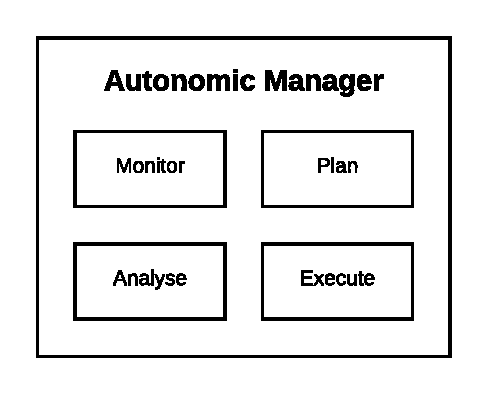
\includegraphics[scale=1]{images/02_theoretical_foundation/autonomic_computing/autonomic_manager}
\caption{Autonomic manager - Source: Authors own model, based on \cite{Jacob2004AutonomicSolution}.}
\label{fig:ac_manager}
\end{figure}

% WHat is the autonomic manager
The autonomic manager implements the control-loop to collect, aggregate, filter and report system metrics from the managed resources. It can only make adjustments within its scope and uses predefined policies to decide what actions have to be executed to accommodate the goals and objectives \cite{Murch2004Autonomic, Sinreich2006AnAB}.
% Knowledge
In addition, the autonomic manager gains knowledge through analysing the managed resources \cite{Murch2004Autonomic}.
% MAPE
The autonomic computing concept digests the MAPE model to implement an autonomic manager, as illustrated in \Fig{fig:ac_manager} \cite{Goscinski2011CloudComputing}.

\begin{itemize}
\item Monitor:
The monitor phase is responsible for collecting the needed metrics from all managed resources and applies aggregation and filter operations to the collected data \cite{Sinreich2006AnAB}.

\item Analyze:
The autonomic manager has to gain knowledge to determine if changes have to be made to the environment \cite{Sinreich2006AnAB}. To predict future situations, the autonomic manager can model complex situations given the collected knowledge \cite{Jacob2004AutonomicSolution}.

\item Plan:
Plans have to be structured to achieve defined goals and objectives. A plan consists of policy-based actions \cite{Jacob2004AutonomicSolution, Sinreich2006AnAB}.

\item Execute:
The execute phase applies all necessary changes to the computing system \cite{Sinreich2006AnAB}.
\end{itemize}

% Multiple manager
Multiple autonomic managers can exist in an autonomic computing environment to perform only certain phases. For example, an autonomic manager which is responsible to monitor and analyse the system and an autonomic manager to plan and execute. To create a complete and closed control-loop, multiple autonomic managers can be composed together \cite{Sinreich2006AnAB}.


% ===========================================
% ===========================================
\section{Performance Metrics}
% Short description
Performance metrics are statistics that describe the system's performance. These statistics are generated by the system, applications, or other tools \cite{Greg2020SysPerf}.
% Common types
Common types for performance metrics are:
\begin{itemize}
\item Throughput: Volume of data or operations per second \cite{Greg2020SysPerf}.
\item Latency: Time of operation \cite{Greg2020SysPerf}.
\item Utilization: Usage of a hardware resource \cite{Greg2020SysPerf}.
\end{itemize}


% Overhead
\paragraph{}It is important to note that measuring performance metrics can cause an overhead. To gather and store performance metrics, additional CPU cycles must be spent. This can have a negative effect on the target performance \cite{Greg2020SysPerf}.


\paragraph{}
% What is utilization
Utilization is a performance metric that describes the usage of a device, e.g., CPU device usage.
% What about time-based utilization
A time-based utilization describes a component's usage during a period where the component was actively performing work \cite{Greg2020SysPerf}.


% 100 utilization
The performance of a hardware resource can degrade significantly if the utilization approaches 100\%.
% Parallel hardware
Hardware that can perform work in parallel might not have a performance degrade at 100\%. That hardware can accept additional work at a high utilization at a later time \cite{Greg2020SysPerf}.


% ===========================================
% ===========================================
\section{Monitoring}
\label{sec:02_monitoring}
% What is monitoring
Monitoring is a process that aims to detect and take care of system faults. In a dynamic environment, becoming aware of the system is a trivial process \cite{Ligus2012EffMonitoring}.
% What is a monitoring system
A monitoring system consists of multiple components responsible for performing measurements on components in the computing environment and collecting, storing, and interpreting the monitored data \cite{Ligus2012EffMonitoring}. 


% The monitoring Loop/Process
\begin{figure}[h]
\centering
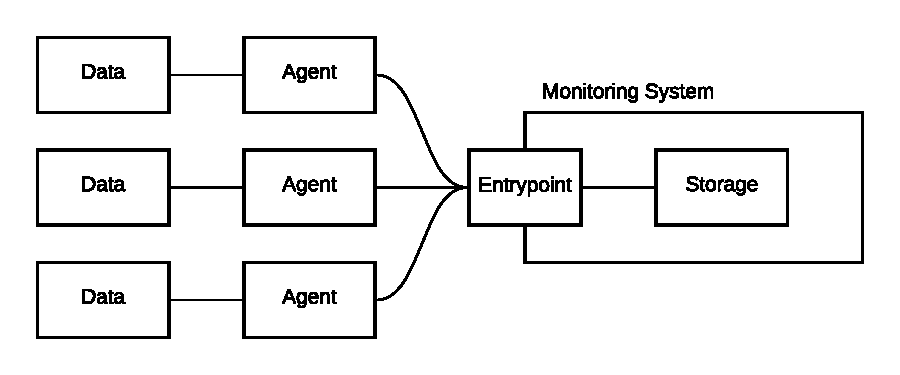
\includegraphics[scale=0.9]{images/02_theoretical_foundation/monitoring/monitoring_system}
\caption{The monitoring process}
\label{fig:mon_mon-system-process}
\end{figure}
In the monitoring process, illustrated in \Fig{fig:mon_mon-system-process}, data is continuously collected by agents. An agent is a process that continuously gathers data from a target. The data can be device statistics, logs, or system measurements. A pull-based monitoring system pulls the data from all specified agents. In contrast, push-based monitoring expects data to be pushed from agents. These two approaches are described in \Sec{subsec:02_monitoring_push-pull}. After the monitoring system has received the data, it groups the data into metrics and stores the metrics in its database \cite{Ligus2012EffMonitoring}.


% Requirements of a monitoring system
The requirements for a monitoring system that can monitor a dynamic changing environment are the following:
\begin{itemize}
\item An efficient database to store metrics \cite{Farcic2017Toolkit21}
\item A push or pull-based way of gathering metrics \cite{Farcic2017Toolkit21}
\item A multi-dimensional data-model \cite{Farcic2017Toolkit21}
\item A powerful query language \cite{Farcic2017Toolkit21}
\end{itemize}


\subsection{Database}
% Continuous data
Continuous data needs to be stored in the most efficient way.
% TSDB
Time-series databases (TSDB) are optimized to store and retrieve time-series data.
% Format
In a time-series database, metrics will be stored in a compact and optimized format. This allows the database to store a massive amount of time-series data on a single machine.


\subsection{Push- and Pull-Based Monitoring Systems}
\label{subsec:02_monitoring_push-pull}
The approach, how the monitoring systems gather metrics to store in the database, plays a significant role.
% There are push and pull based systems
Push- and pull-based systems are the two primary approaches to gather metrics from services.
% About push
Push-based monitoring systems expect services to push metrics to their storage.
% About pull
Pull-based monitoring systems scrape metrics from all defined targets. Targets do not know about the monitoring system's existence and only need to collect and expose metrics \cite{Farcic2017Toolkit21}.


% When to choose what (Discovery)
Service discovery is an important aspect to decide whenever to use a pull- or push-based monitoring system \cite{Farcic2017Toolkit21}.

\begin{figure}[h]
\centering
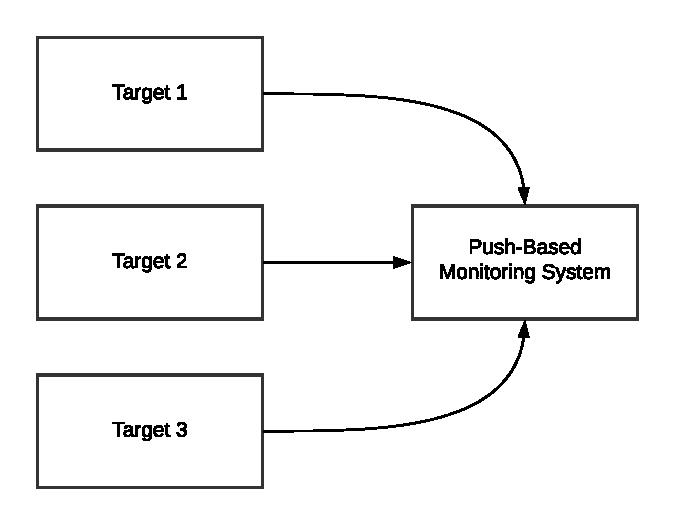
\includegraphics[scale=0.8]{images/02_theoretical_foundation/monitoring/push_based}
\caption{Push-based monitoring approach}
\label{fig:mon_push-based}
\end{figure}
% Push based discovery
In a push-based environment, services only need to know the monitoring service's address to push their data to the storage \cite{Farcic2017Toolkit21}.


\begin{figure}[h]
\centering
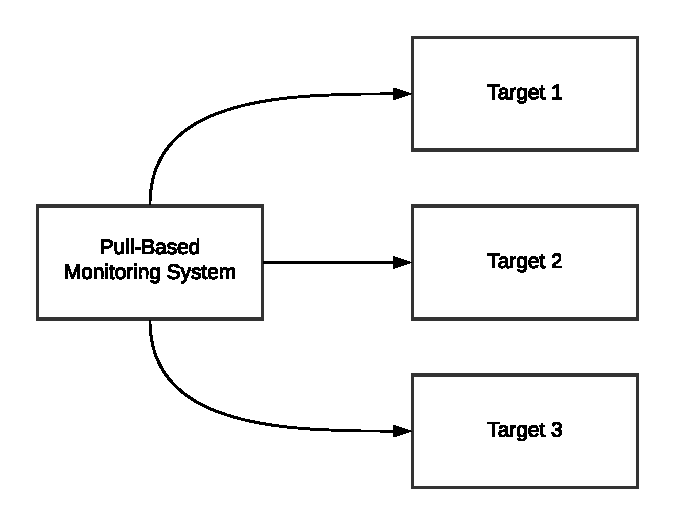
\includegraphics[scale=0.8]{images/02_theoretical_foundation/monitoring/pull_based}
\caption{Pull-based monitoring approach}
\label{fig:mon_pull-based}
\end{figure}
% Pull based discovery
A pull-based monitoring tool needs to know the address of each target in the environment.
% Why pull based works best with discovery
The advantage of a pull-based monitoring system is the simplicity to detect whenever a target has failed or is not available \cite{Farcic2017Toolkit21}.


\subsection{Multi-Dimensional Data Model}
\label{subsec:02_monitoring_db_multi-model}
% Intro
Metrics are store as time-series data, where a time-series is a combination of a name and a set of optional key-value pairs called labels.
% The name
The name of a time-series identifies the metric which is measured.
% Labels
Labels provide a multi-dimensional data-model to the stored data. Each combination of labels represents a specific dimensional instantiation of a metric \cite{Prom2020Docs}.
% Dynamic env
In a dynamic environment, services are dynamically added and removed. Therefore, a dynamic environment needs a multi-dimensional data model to represent all dimensions in the environment \cite{Farcic2018Toolkit22}.
% A query language
A powerful query language that provides capabilities to perform aggregations and filtering on dimensions is needed in addition to a multi-dimensional data model.
% Example
\begin{lstlisting}[label=lst:02_monitoring_db_multi-model_metr_dimless, caption=Example of a dimensionless-metric, numbers=none]
container_cpu_user_seconds_total
\end{lstlisting}
\begin{lstlisting}[label=lst:02_monitoring_db_multi-model_metr_withdim, caption=Example of a metric with dimensions, numbers=none]
container_cpu_user_seconds_total{image="spark-worker:3.0.1-hadoop2.7"}
\end{lstlisting}
% Explain
\Lst{lst:02_monitoring_db_multi-model_metr_dimless} provides an example of a metric without labels, and \Lst{lst:02_monitoring_db_multi-model_metr_withdim} shows an example of a metric with a label. As the examples show, The metric with a label provides more efficient querying to gather specific information about a metric.
